
%% bare_conf.tex
%% V1.4b
%% 2015/08/26
%% by Michael Shell
%% See:
%% http://www.michaelshell.org/
%% for current contact information.
%%
%% This is a skeleton file demonstrating the use of IEEEtran.cls
%% (requires IEEEtran.cls version 1.8b or later) with an IEEE
%% conference paper.
%%
%% Support sites:
%% http://www.michaelshell.org/tex/ieeetran/
%% http://www.ctan.org/pkg/ieeetran
%% and
%% http://www.ieee.org/

%%*************************************************************************
%% Legal Notice:
%% This code is offered as-is without any warranty either expressed or
%% implied; without even the implied warranty of MERCHANTABILITY or
%% FITNESS FOR A PARTICULAR PURPOSE! 
%% User assumes all risk.
%% In no event shall the IEEE or any contributor to this code be liable for
%% any damages or losses, including, but not limited to, incidental,
%% consequential, or any other damages, resulting from the use or misuse
%% of any information contained here.
%%
%% All comments are the opinions of their respective authors and are not
%% necessarily endorsed by the IEEE.
%%
%% This work is distributed under the LaTeX Project Public License (LPPL)
%% ( http://www.latex-project.org/ ) version 1.3, and may be freely used,
%% distributed and modified. A copy of the LPPL, version 1.3, is included
%% in the base LaTeX documentation of all distributions of LaTeX released
%% 2003/12/01 or later.
%% Retain all contribution notices and credits.
%% ** Modified files should be clearly indicated as such, including  **
%% ** renaming them and changing author support contact information. **
%%*************************************************************************


% *** Authors should verify (and, if needed, correct) their LaTeX system  ***
% *** with the testflow diagnostic prior to trusting their LaTeX platform ***
% *** with production work. The IEEE's font choices and paper sizes can   ***
% *** trigger bugs that do not appear when using other class files.       ***                          ***
% The testflow support page is at:
% http://www.michaelshell.org/tex/testflow/



\documentclass[conference]{IEEEtran}

\usepackage{csquotes}
\usepackage{graphicx}
\usepackage{booktabs}
\usepackage{caption}
\usepackage{threeparttable}
\usepackage{adjustbox}
\usepackage{multicol}
\graphicspath{ {images/} }
% Some Computer Society conferences also require the compsoc mode option,
% but others use the standard conference format.
%
% If IEEEtran.cls has not been installed into the LaTeX system files,
% manually specify the path to it like:
% \documentclass[conference]{../sty/IEEEtran}





% Some very useful LaTeX packages include:
% (uncomment the ones you want to load)


% *** MISC UTILITY PACKAGES ***
%
%\usepackage{ifpdf}
% Heiko Oberdiek's ifpdf.sty is very useful if you need conditional
% compilation based on whether the output is pdf or dvi.
% usage:
% \ifpdf
%   % pdf code
% \else
%   % dvi code
% \fi
% The latest version of ifpdf.sty can be obtained from:
% http://www.ctan.org/pkg/ifpdf
% Also, note that IEEEtran.cls V1.7 and later provides a builtin
% \ifCLASSINFOpdf conditional that works the same way.
% When switching from latex to pdflatex and vice-versa, the compiler may
% have to be run twice to clear warning/error messages.






% *** CITATION PACKAGES ***
%
%\usepackage{cite}
% cite.sty was written by Donald Arseneau
% V1.6 and later of IEEEtran pre-defines the format of the cite.sty package
% \cite{} output to follow that of the IEEE. Loading the cite package will
% result in citation numbers being automatically sorted and properly
% "compressed/ranged". e.g., [1], [9], [2], [7], [5], [6] without using
% cite.sty will become [1], [2], [5]--[7], [9] using cite.sty. cite.sty's
% \cite will automatically add leading space, if needed. Use cite.sty's
% noadjust option (cite.sty V3.8 and later) if you want to turn this off
% such as if a citation ever needs to be enclosed in parenthesis.
% cite.sty is already installed on most LaTeX systems. Be sure and use
% version 5.0 (2009-03-20) and later if using hyperref.sty.
% The latest version can be obtained at:
% http://www.ctan.org/pkg/cite
% The documentation is contained in the cite.sty file itself.






% *** GRAPHICS RELATED PACKAGES ***
%
\ifCLASSINFOpdf
  % \usepackage[pdftex]{graphicx}
  % declare the path(s) where your graphic files are
  % \graphicspath{{../pdf/}{../jpeg/}}
  % and their extensions so you won't have to specify these with
  % every instance of \includegraphics
  % \DeclareGraphicsExtensions{.pdf,.jpeg,.png}
\else
  % or other class option (dvipsone, dvipdf, if not using dvips). graphicx
  % will default to the driver specified in the system graphics.cfg if no
  % driver is specified.
  % \usepackage[dvips]{graphicx}
  % declare the path(s) where your graphic files are
  % \graphicspath{{../eps/}}
  % and their extensions so you won't have to specify these with
  % every instance of \includegraphics
  % \DeclareGraphicsExtensions{.eps}
\fi
% graphicx was written by David Carlisle and Sebastian Rahtz. It is
% required if you want graphics, photos, etc. graphicx.sty is already
% installed on most LaTeX systems. The latest version and documentation
% can be obtained at: 
% http://www.ctan.org/pkg/graphicx
% Another good source of documentation is "Using Imported Graphics in
% LaTeX2e" by Keith Reckdahl which can be found at:
% http://www.ctan.org/pkg/epslatex
%
% latex, and pdflatex in dvi mode, support graphics in encapsulated
% postscript (.eps) format. pdflatex in pdf mode supports graphics
% in .pdf, .jpeg, .png and .mps (metapost) formats. Users should ensure
% that all non-photo figures use a vector format (.eps, .pdf, .mps) and
% not a bitmapped formats (.jpeg, .png). The IEEE frowns on bitmapped formats
% which can result in "jaggedy"/blurry rendering of lines and letters as
% well as large increases in file sizes.
%
% You can find documentation about the pdfTeX application at:
% http://www.tug.org/applications/pdftex





% *** MATH PACKAGES ***
%
%\usepackage{amsmath}
% A popular package from the American Mathematical Society that provides
% many useful and powerful commands for dealing with mathematics.
%
% Note that the amsmath package sets \interdisplaylinepenalty to 10000
% thus preventing page breaks from occurring within multiline equations. Use:
%\interdisplaylinepenalty=2500
% after loading amsmath to restore such page breaks as IEEEtran.cls normally
% does. amsmath.sty is already installed on most LaTeX systems. The latest
% version and documentation can be obtained at:
% http://www.ctan.org/pkg/amsmath





% *** SPECIALIZED LIST PACKAGES ***
%
%\usepackage{algorithmic}
% algorithmic.sty was written by Peter Williams and Rogerio Brito.
% This package provides an algorithmic environment fo describing algorithms.
% You can use the algorithmic environment in-text or within a figure
% environment to provide for a floating algorithm. Do NOT use the algorithm
% floating environment provided by algorithm.sty (by the same authors) or
% algorithm2e.sty (by Christophe Fiorio) as the IEEE does not use dedicated
% algorithm float types and packages that provide these will not provide
% correct IEEE style captions. The latest version and documentation of
% algorithmic.sty can be obtained at:
% http://www.ctan.org/pkg/algorithms
% Also of interest may be the (relatively newer and more customizable)
% algorithmicx.sty package by Szasz Janos:
% http://www.ctan.org/pkg/algorithmicx




% *** ALIGNMENT PACKAGES ***
%
%\usepackage{array}
% Frank Mittelbach's and David Carlisle's array.sty patches and improves
% the standard LaTeX2e array and tabular environments to provide better
% appearance and additional user controls. As the default LaTeX2e table
% generation code is lacking to the point of almost being broken with
% respect to the quality of the end results, all users are strongly
% advised to use an enhanced (at the very least that provided by array.sty)
% set of table tools. array.sty is already installed on most systems. The
% latest version and documentation can be obtained at:
% http://www.ctan.org/pkg/array


% IEEEtran contains the IEEEeqnarray family of commands that can be used to
% generate multiline equations as well as matrices, tables, etc., of high
% quality.




% *** SUBFIGURE PACKAGES ***
%\ifCLASSOPTIONcompsoc
%  \usepackage[caption=false,font=normalsize,labelfont=sf,textfont=sf]{subfig}
%\else
%  \usepackage[caption=false,font=footnotesize]{subfig}
%\fi
% subfig.sty, written by Steven Douglas Cochran, is the modern replacement
% for subfigure.sty, the latter of which is no longer maintained and is
% incompatible with some LaTeX packages including fixltx2e. However,
% subfig.sty requires and automatically loads Axel Sommerfeldt's caption.sty
% which will override IEEEtran.cls' handling of captions and this will result
% in non-IEEE style figure/table captions. To prevent this problem, be sure
% and invoke subfig.sty's "caption=false" package option (available since
% subfig.sty version 1.3, 2005/06/28) as this is will preserve IEEEtran.cls
% handling of captions.
% Note that the Computer Society format requires a larger sans serif font
% than the serif footnote size font used in traditional IEEE formatting
% and thus the need to invoke different subfig.sty package options depending
% on whether compsoc mode has been enabled.
%
% The latest version and documentation of subfig.sty can be obtained at:
% http://www.ctan.org/pkg/subfig




% *** FLOAT PACKAGES ***
%
%\usepackage{fixltx2e}
% fixltx2e, the successor to the earlier fix2col.sty, was written by
% Frank Mittelbach and David Carlisle. This package corrects a few problems
% in the LaTeX2e kernel, the most notable of which is that in current
% LaTeX2e releases, the ordering of single and double column floats is not
% guaranteed to be preserved. Thus, an unpatched LaTeX2e can allow a
% single column figure to be placed prior to an earlier double column
% figure.
% Be aware that LaTeX2e kernels dated 2015 and later have fixltx2e.sty's
% corrections already built into the system in which case a warning will
% be issued if an attempt is made to load fixltx2e.sty as it is no longer
% needed.
% The latest version and documentation can be found at:
% http://www.ctan.org/pkg/fixltx2e


%\usepackage{stfloats}
% stfloats.sty was written by Sigitas Tolusis. This package gives LaTeX2e
% the ability to do double column floats at the bottom of the page as well
% as the top. (e.g., "\begin{figure*}[!b]" is not normally possible in
% LaTeX2e). It also provides a command:
%\fnbelowfloat
% to enable the placement of footnotes below bottom floats (the standard
% LaTeX2e kernel puts them above bottom floats). This is an invasive package
% which rewrites many portions of the LaTeX2e float routines. It may not work
% with other packages that modify the LaTeX2e float routines. The latest
% version and documentation can be obtained at:
% http://www.ctan.org/pkg/stfloats
% Do not use the stfloats baselinefloat ability as the IEEE does not allow
% \baselineskip to stretch. Authors submitting work to the IEEE should note
% that the IEEE rarely uses double column equations and that authors should try
% to avoid such use. Do not be tempted to use the cuted.sty or midfloat.sty
% packages (also by Sigitas Tolusis) as the IEEE does not format its papers in
% such ways.
% Do not attempt to use stfloats with fixltx2e as they are incompatible.
% Instead, use Morten Hogholm'a dblfloatfix which combines the features
% of both fixltx2e and stfloats:
%
% \usepackage{dblfloatfix}
% The latest version can be found at:
% http://www.ctan.org/pkg/dblfloatfix




% *** PDF, URL AND HYPERLINK PACKAGES ***
%
%\usepackage{url}
% url.sty was written by Donald Arseneau. It provides better support for
% handling and breaking URLs. url.sty is already installed on most LaTeX
% systems. The latest version and documentation can be obtained at:
% http://www.ctan.org/pkg/url
% Basically, \url{my_url_here}.




% *** Do not adjust lengths that control margins, column widths, etc. ***
% *** Do not use packages that alter fonts (such as pslatex).         ***
% There should be no need to do such things with IEEEtran.cls V1.6 and later.
% (Unless specifically asked to do so by the journal or conference you plan
% to submit to, of course. )


% correct bad hyphenation here
\hyphenation{op-tical net-works semi-conduc-tor}


\begin{document}
%
% paper title
% Titles are generally capitalized except for words such as a, an, and, as,
% at, but, by, for, in, nor, of, on, or, the, to and up, which are usually
% not capitalized unless they are the first or last word of the title.
% Linebreaks \\ can be used within to get better formatting as desired.
% Do not put math or special symbols in the title.
\title{Predicting and visualising ATM attacks}


% author names and affiliations
% use a multiple column layout for up to three different
% affiliations
\author{\IEEEauthorblockN{R. Fasel and B. Regnerus}
\IEEEauthorblockA{Faculty of Electrical Engineering, Mathematics and Computer Science \\
University of Twente\\
7500 AE Enschede, The Netherlands}}


% conference papers do not typically use \thanks and this command
% is locked out in conference mode. If really needed, such as for
% the acknowledgment of grants, issue a \IEEEoverridecommandlockouts
% after \documentclass

% for over three affiliations, or if they all won't fit within the width
% of the page, use this alternative format:
% 
%\author{\IEEEauthorblockN{Michael Shell\IEEEauthorrefmark{1},
%Homer Simpson\IEEEauthorrefmark{2},
%James Kirk\IEEEauthorrefmark{3}, 
%Montgomery Scott\IEEEauthorrefmark{3} and
%Eldon Tyrell\IEEEauthorrefmark{4}}
%\IEEEauthorblockA{\IEEEauthorrefmark{1}School of Electrical and Computer Engineering\\
%Georgia Institute of Technology,
%Atlanta, Georgia 30332--0250\\ Email: see http://www.michaelshell.org/contact.html}
%\IEEEauthorblockA{\IEEEauthorrefmark{2}Twentieth Century Fox, Springfield, USA\\
%Email: homer@thesimpsons.com}
%\IEEEauthorblockA{\IEEEauthorrefmark{3}Starfleet Academy, San Francisco, California 96678-2391\\
%Telephone: (800) 555--1212, Fax: (888) 555--1212}
%\IEEEauthorblockA{\IEEEauthorrefmark{4}Tyrell Inc., 123 Replicant Street, Los Angeles, California 90210--4321}}




% use for special paper notices
%\IEEEspecialpapernotice{(Invited Paper)}




% make the title area
\maketitle


% no keywords




% For peer review papers, you can put extra information on the cover
% page as needed:
% \ifCLASSOPTIONpeerreview
% \begin{center} \bfseries EDICS Category: 3-BBND \end{center}
% \fi
%
% For peerreview papers, this IEEEtran command inserts a page break and
% creates the second title. It will be ignored for other modes.
\IEEEpeerreviewmaketitle



\section{Introduction} \label{introduction}
% no \IEEEPARstart

ATM attacks and fraud continue to make headlines. The compromise of ATMs is a very lucrative criminal business. ATMs typically exist as physical contact points of the banking infrastructure that are exposed to public sight. This makes ATMs a very accessible target for exploitation, vulnerable to a large variety of attack scenarios. The European ATM Security Team report that the amount of ATM attacks both physical- and logical attacks only increase \cite{c1}, therefore securing ATMs but also predicting ATM attacks are more important then ever.

This paper describes the process of both visualising ATM attacks and predicting cases where ATM attacks could occur. The main focus of this of this research is the exploration of using tools provided in the DM- and DPV topics provided in the Data Science course. Furthermore other tools such as the Python machine learning library Scikit-learn and JavaScript data visualisation library D3.js will be used.

\subsection{The Dataset}
Provided for this project is a dataset from the European TREsPASS project  \cite{c2} that was developed in collaboration with Spanish banks. The dataset contains information of 723 ATMs, attacks on those ATMs and the information about those attacks. In more detail, the dataset provides: geographical details about ATMs (such as latitude and longitude coordinates, distance to a highway), demographic details (such as per capita income, population density, median population age), logging details of the attacks per ATM, the profile of the involved attacker, the information on how much amount was recovered and when did recovery event took place.

For this research the most important features of the dataset are both the geographical- and demographical features. Those features can be used for both visualising attacks and predicting attacks using a classifier with those features as an input.

\subsection{Research Questions} \label{questions}

With the DataScience DM and DPV topics in mind this lead to the following research questions:

\begin{displayquote}
	How can a dataset containing geographical- and demographical features of ATM attacks be predicted and visualised?
\end{displayquote}

This question is answered with the support of the following questions:  

\begin{itemize}
\item How can factors that contribute to attack frequency and attacker success be plotted geographically?
\item Which factors contribute most to attack frequency and attacker success?
\item How can ATM attacks be predicted using a Naive Bayes classifier?

\end{itemize}


% An example of a floating figure using the graphicx package.
% Note that \label must occur AFTER (or within) \caption.
% For figures, \caption should occur after the \includegraphics.
% Note that IEEEtran v1.7 and later has special internal code that
% is designed to preserve the operation of \label within \caption
% even when the captionsoff option is in effect. However, because
% of issues like this, it may be the safest practice to put all your
% \label just after \caption rather than within \caption{}.
%
% Reminder: the "draftcls" or "draftclsnofoot", not "draft", class
% option should be used if it is desired that the figures are to be
% displayed while in draft mode.
%
%\begin{figure}[!t]
%\centering
%\includegraphics[width=2.5in]{myfigure}
% where an .eps filename suffix will be assumed under latex, 
% and a .pdf suffix will be assumed for pdflatex; or what has been declared
% via \DeclareGraphicsExtensions.
%\caption{Simulation results for the network.}
%\label{fig_sim}
%\end{figure}

% Note that the IEEE typically puts floats only at the top, even when this
% results in a large percentage of a column being occupied by floats.


% An example of a double column floating figure using two subfigures.
% (The subfig.sty package must be loaded for this to work.)
% The subfigure \label commands are set within each subfloat command,
% and the \label for the overall figure must come after \caption.
% \hfil is used as a separator to get equal spacing.
% Watch out that the combined width of all the subfigures on a 
% line do not exceed the text width or a line break will occur.
%
%\begin{figure*}[!t]
%\centering
%\subfloat[Case I]{\includegraphics[width=2.5in]{box}%
%\label{fig_first_case}}
%\hfil
%\subfloat[Case II]{\includegraphics[width=2.5in]{box}%
%\label{fig_second_case}}
%\caption{Simulation results for the network.}
%\label{fig_sim}
%\end{figure*}
%
% Note that often IEEE papers with subfigures do not employ subfigure
% captions (using the optional argument to \subfloat[]), but instead will
% reference/describe all of them (a), (b), etc., within the main caption.
% Be aware that for subfig.sty to generate the (a), (b), etc., subfigure
% labels, the optional argument to \subfloat must be present. If a
% subcaption is not desired, just leave its contents blank,
% e.g., \subfloat[].


% An example of a floating table. Note that, for IEEE style tables, the
% \caption command should come BEFORE the table and, given that table
% captions serve much like titles, are usually capitalized except for words
% such as a, an, and, as, at, but, by, for, in, nor, of, on, or, the, to
% and up, which are usually not capitalized unless they are the first or
% last word of the caption. Table text will default to \footnotesize as
% the IEEE normally uses this smaller font for tables.
% The \label must come after \caption as always.
%
%\begin{table}[!t]
%% increase table row spacing, adjust to taste
%\renewcommand{\arraystretch}{1.3}
% if using array.sty, it might be a good idea to tweak the value of
% \extrarowheight as needed to properly center the text within the cells
%\caption{An Example of a Table}
%\label{table_example}
%\centering
%% Some packages, such as MDW tools, offer better commands for making tables
%% than the plain LaTeX2e tabular which is used here.
%\begin{tabular}{|c||c|}
%\hline
%One & Two\\
%\hline
%Three & Four\\
%\hline
%\end{tabular}
%\end{table}


% Note that the IEEE does not put floats in the very first column
% - or typically anywhere on the first page for that matter. Also,
% in-text middle ("here") positioning is typically not used, but it
% is allowed and encouraged for Computer Society conferences (but
% not Computer Society journals). Most IEEE journals/conferences use
% top floats exclusively. 
% Note that, LaTeX2e, unlike IEEE journals/conferences, places
% footnotes above bottom floats. This can be corrected via the
% \fnbelowfloat command of the stfloats package.


\section{Method} \label{method}
To give an accurate answer the above mentioned research questions multiple different tasks have to be conducted. The tasks have been further separated in the application of topic DPV (\ref{dpv}) and the application of topic DM (\ref{dm}).

\subsection{Application of Topic DPV} \label{dpv}
In this section we try to identify a good method for obtaining visualisation from the raw ATM attack dataset. Raw data was available in an ARFF format and a good description of each data column was also available. The data which was available was already in quite a clear format and did not need many transformations to make it available for visualisation. Therefore Pentaho Kettle was not used, instead basic transformations were performed to transform the ARFF file to a GeoJSON format using the Python language, since the data which is encoded consists of geographic data points this format seemed appropriate. For the visualisation we wanted to also show the contours of the freguesias (municipalities of Lisbon). This data was not available in the ATM attack dataset, however it was available under an Creative Commons licence from the Lisbon Open Data website \cite{c4}.

Using the two GeoJSON formatted datasets a visualisation was created in Javascript using D3.js. \cite{c5} The use of the D3.js library was chosen over other tools such as Tableau since it allows for more flexibility when developing visualisations. D3.js is able to read from the GeoJSON formatted files, using them as the datasource therefore no external database warehouse, such as MySQL, was needed. 

\subsection{Application of Topic DM} \label{dm}
A Naive Bayes (NB) classifier was created in order to predict ATM attacks. Naive Bayes classifiers provide probabilities for each class, in this case attacked or not attacked. These probabilities can be used to give an accurate prediction of the probability of an ATM attack.
The Naive Bayes classifier was created using the Scikit-learn library for the Python programming language. Scikit-learn is a library that provides tools to setup, test and evaluate Machine learning algorithms. 
The NB classifier was trained using the data available from *INSERT LINK ETC*. The data consisted of ATM records that described properties of the ATM and most importantly if they were attacked and how many times. The class label was extracted from the variable 'N_FREQ_ATK' which indicates if a ATM was attacked or not. Together with the class labels some features were selected from the ATM properties. These features included: *INSTER FEATURES*. 



\section{Results} \label{results}
Following from \ref{method} (the method) a visualisation was developed in D3.js (\ref{dpvres}) together with a machine learning model created using a Naive Bayes classification method (\ref{dmres}).

\subsection{Results of Topic DPV} \label{dpvres}
The visualisation which was developed contains the outlines of the freguesias as a grey shape, on top of those shapes the ATMs are plotted geographically as black dots. ATMs which have been attacked have a red circle around them. The visualisation can be further explored by turning on- and off other visualisation layers. There can be chosen from a list of nine different features that will be visualised as circles on the map. Most prominently, the predicted attack probability can be visualised, this probability is the outcome of \ref{dm} (the Application of Topic DM) and will be further discussed in \ref{dmres} (Results of Topic DM). Other features that can be displayed are, inter alia, motorway distance, or police distance. These features were all present in the ATM attacks dataset. The scale of the circles is explained by a circle legend giving the values of the corresponding circle size. The source code and full visualisation can be found on Github \cite{c3}\cite{c6}.

{
\centering
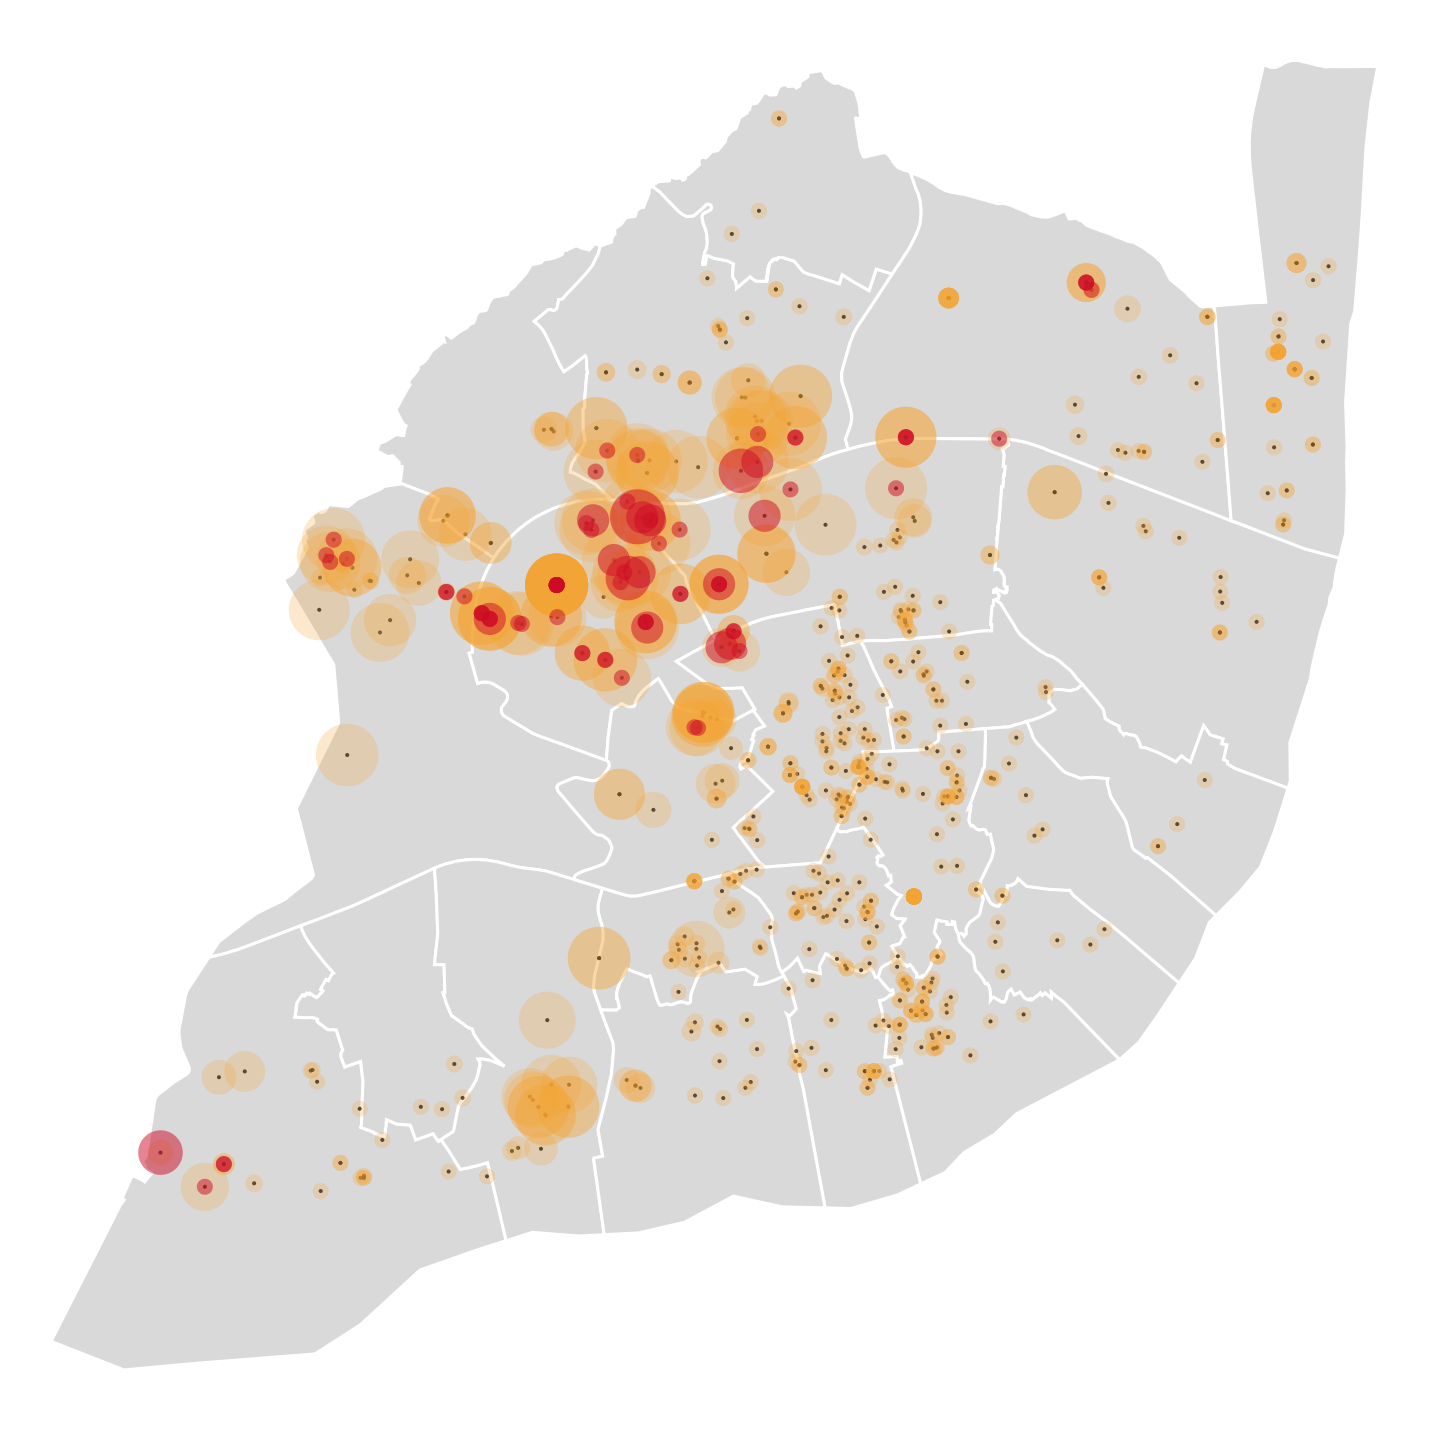
\includegraphics[width=0.95\linewidth]{visualisation.png}\\
\captionof{figure}{Visualisation of ATM attacks (red circles), Predicted ATM attacks (orange circles) and ATM locations (black dots) on the map of Lisbon. \cite{c3}}\label{fig:confusion}
}


\subsection{Results of Topic DM} \label{dmres}
(TODO)

{
\begin{center}
\centering
\captionof{table}{Performance results}\label{fig:results}
\begin{tabular}{@{}lllll@{}}
\toprule
& Precision & Recall & F1-score & Support                  
\\ \midrule
\multicolumn{1}{|l|}{XX}  & 
\multicolumn{1}{l|}{0\%} & 
\multicolumn{1}{l|}{0\%} & 
\multicolumn{1}{l|}{0\%} & 
\multicolumn{1}{l|}{0} 
\\ \midrule

\multicolumn{1}{|l|}{XX} & 
\multicolumn{1}{l|}{0\%} & 
\multicolumn{1}{l|}{0\%} & 
\multicolumn{1}{l|}{0\%} & 
\multicolumn{1}{l|}{0} 

\\ \midrule
avg / total & 0\% & 0\% & 0\% & 0                      

\\ \bottomrule
\end{tabular}
\end{center}
}

\section{Conclusion and Discussion} \label{results}
According to the results from both the data visualisation and machine learning prediction, it is possible to accurately predict locations for ATM attacks and visualise the attacks with the geographical- and demographical features provided by the ATM attacks dataset.

Since the data was labeled with latitude and longitude coordinates the visualisation created in D3.js proves that it is possible to plot attack frequency and attacker success geographically. There are however a few drawbacks from the visualisation. Since some locations, for example a bank, have multiple ATMs at the same location, the circles overlap and therefore can distort the visualisation. In addition all features are labeled to a specific ATM location, therefore some locations have a lot of demographical data available while other places have little data available.

(EXPLAIN FACTORS WHICH CONTRIBUTE TO ATTACKS)

(EXPLAIN RESULTS CLASSIFIER)

Further research should be done to optimise the machine learning model even further. More datasources could be sourced as input features for the model. Furthermore there could be experimented with other types of classifiers to further improve the classification.


% trigger a \newpage just before the given reference
% number - used to balance the columns on the last page
% adjust value as needed - may need to be readjusted if
% the document is modified later
%\IEEEtriggeratref{8}
% The "triggered" command can be changed if desired:
%\IEEEtriggercmd{\enlargethispage{-5in}}

% references section

% can use a bibliography generated by BibTeX as a .bbl file
% BibTeX documentation can be easily obtained at:
% http://mirror.ctan.org/biblio/bibtex/contrib/doc/
% The IEEEtran BibTeX style support page is at:
% http://www.michaelshell.org/tex/ieeetran/bibtex/
%\bibliographystyle{IEEEtran}
% argument is your BibTeX string definitions and bibliography database(s)
%\bibliography{IEEEabrv,../bib/paper}
%
% <OR> manually copy in the resultant .bbl file
% set second argument of \begin to the number of references
% (used to reserve space for the reference number labels box)
\begin{thebibliography}{1}

\bibitem{c1}
“European ATM Crime Report Archives | European ATM Security Team,” European ATM Security Team. [Online]. Available: https://www.european-atm-security.eu/tag/european-atm-crime-report/. [Accessed: 13-Apr-2017]
\bibitem{c2} 
“The TREsPASS Project.” [Online]. Available: https://www.trespass-project.eu. [Accessed: 13-Apr-2017]
\bibitem{c3}
“ATM Attacks.” [Online]. Available: https://regnerus.github.io/atm-attack-data-visualisation/. [Accessed: 13-Apr-2017]
\bibitem{c4}
“Câmara Municipal de Lisboa - Organisationer - Portal Dados Abertos.” [Online]. Available: http://dados.cm-lisboa.pt/sv/organization/camara-municipal-de-lisboa. [Accessed: 14-Apr-2017]
\bibitem{c5} 
M. Bostock, “D3.js - Data-Driven Documents.” [Online]. Available: https://d3js.org/. [Accessed: 14-Apr-2017]
\bibitem{c6}
regnerus, “regnerus/atm-attack-data-visualisation,” GitHub. [Online]. Available: https://github.com/regnerus/atm-attack-data-visualisation. [Accessed: 14-Apr-2017]


\end{thebibliography}




% that's all folks
\end{document}


